% latbibdo  templateApJ

\newcommand\apjcls{1}
\newcommand\aastexcls{2}
\newcommand\othercls{3}

% Select ony one of the following \papercls and cls file:

% Emulate ApJ cls:
%\newcommand\papercls{\apjcls}
%\documentclass[iop]{emulateapj}

% AASTEX6 cls:
\newcommand\papercls{\aastexcls}
\documentclass[tighten, times, preprint2]{aastex6}  % ApJ look-alike
%\documentclass[tighten, times, manuscript]{aastex6} % Onecolumn, doublespaced

% Other cls:
%\newcommand\papercls{\othercls}
%\documentclass[letterpaper,12pt]{article}
%\documentclass[12pt,preprint]{aastex}
%\documentclass[letterpaper,12pt]{article}

% These are latex packages that enable various capability.
% Google to find out about each one, and look in the README.
\if\papercls \apjcls
\usepackage{apjfonts}
\else\if\papercls \othercls
\usepackage{epsfig}
\fi\fi
\usepackage{ifthen}
\usepackage{natbib}
\usepackage{amssymb, amsmath}
\usepackage{appendix}
\usepackage{etoolbox}
%\usepackage{rotating}
%\usepackage{lscape}

% To have nice and size-adjustable \texttt fonts:
\usepackage[T1]{fontenc}
\usepackage[scaled=.75]{beramono}

% This one defines a few more journals (DPS and AAS abstracts) for bibtex:
\if\papercls \apjcls
\newcommand\aas{\ref@jnl{AAS Meeting Abstracts}}% *** added by jh
          % American Astronomical Society Meeting Abstracts
\newcommand\dps{\ref@jnl{AAS/DPS Meeting Abstracts}}% *** added by jh
          % American Astronomical Society/Division for Planetary Sciences Meeting Abstracts
\newcommand\maps{\ref@jnl{MAPS}}% *** added by jh
          % Meteoritics and Planetary Science
\else\if\papercls \othercls
\usepackage{astjnlabbrev-jh}
\fi\fi

% Bibliographystyle chooses a bibtex .bst file, which defines the
% format of the references.  It's important to pick one that works for
% the journal you are writing for and that has hyperlinks for the
% actual paper online.
\bibliographystyle{apj_hyperref}
%\bibliographystyle{hapj}
%\bibliographystyle{apj}

% \bibpunct sets the punctuation used in citations (year in parens or
% brackets, etc.).  Emulateapj has an error (semicolon instead of
% first comma in braces).  Once that's fixed, take out the first
% \bibpunct line.
\if\papercls \apjcls
\bibpunct[, ]{(}{)}{,}{a}{}{,}
\else
\bibpunct[, ]{(}{)}{,}{a}{}{,}
\fi


% Setup hyperreferences style:
\if\papercls \aastexcls
\hypersetup{citecolor=blue, % color for \cite{...} links
            linkcolor=blue, % color for \ref{...} links
            menucolor=blue, % color for Acrobat menu buttons
            urlcolor=blue}  % color for \url{...} links
\else
\usepackage[%pdftex,      % hyper-references for pdflatex
bookmarks=true,           %%% generate bookmarks ...
bookmarksnumbered=true,   %%% ... with numbers
colorlinks=true,          % links are colored
citecolor=blue,           % color for \cite{...} links
linkcolor=blue,           % color for \ref{...} links
menucolor=blue,           % color for Acrobat menu buttons
urlcolor=blue,            % color for \url{...} links
linkbordercolor={0 0 1},  %%% blue frames around links
pdfborder={0 0 1},
frenchlinks=true]{hyperref}
\fi

% These macross generate the hyperlinks in the References section:
\if\papercls \othercls
\newcommand{\eprint}[1]{\href{http://arxiv.org/abs/#1}{#1}}
\else
\renewcommand{\eprint}[1]{\href{http://arxiv.org/abs/#1}{#1}}
\fi
\newcommand{\ISBN}[1]{\href{http://cosmologist.info/ISBN/#1}{ISBN: #1}}
\providecommand{\adsurl}[1]{\href{#1}{ADS}}

% hyper ref only the year in citations:
\makeatletter
% Patch case where name and year are separated by aysep
\patchcmd{\NAT@citex}
  {\@citea\NAT@hyper@{%
     \NAT@nmfmt{\NAT@nm}%
     \hyper@natlinkbreak{\NAT@aysep\NAT@spacechar}{\@citeb\@extra@b@citeb}%
     \NAT@date}}
  {\@citea\NAT@nmfmt{\NAT@nm}%
   \NAT@aysep\NAT@spacechar\NAT@hyper@{\NAT@date}}{}{}

% Patch case where name and year are separated by opening bracket
\patchcmd{\NAT@citex}
  {\@citea\NAT@hyper@{%
     \NAT@nmfmt{\NAT@nm}%
     \hyper@natlinkbreak{\NAT@spacechar\NAT@@open\if*#1*\else#1\NAT@spacechar\fi}%
       {\@citeb\@extra@b@citeb}%
     \NAT@date}}
  {\@citea\NAT@nmfmt{\NAT@nm}%
   \NAT@spacechar\NAT@@open\if*#1*\else#1\NAT@spacechar\fi\NAT@hyper@{\NAT@date}}
  {}{}
\makeatother

% Define lowcase: a MakeLowercase that doesn't break on subtitles:
\makeatletter
\DeclareRobustCommand{\lowcase}[1]{\@lowcase#1\@nil}
\def\@lowcase#1\@nil{\if\relax#1\relax\else\MakeLowercase{#1}\fi}
\pdfstringdefDisableCommands{\let\lowcase\@firstofone}
\makeatother

% unslanted mu, for ``micro'' abbrev.
\DeclareSymbolFont{UPM}{U}{eur}{m}{n}
\DeclareMathSymbol{\umu}{0}{UPM}{"16}
\let\oldumu=\umu
\renewcommand\umu{\ifmmode\oldumu\else\math{\oldumu}\fi}
\newcommand\micro{\umu}
\if\papercls \othercls
\newcommand\micron{\micro m}
\else
\renewcommand\micron{\micro m}
\fi
\newcommand\microns{\micron}
\newcommand\microbar{\micro bar}

% These define commands outside of math mode:
% \sim
\let\oldsim=\sim
\renewcommand\sim{\ifmmode\oldsim\else\math{\oldsim}\fi}
% \pm
\let\oldpm=\pm
\renewcommand\pm{\ifmmode\oldpm\else\math{\oldpm}\fi}
% \times
\newcommand\by{\ifmmode\times\else\math{\times}\fi}
% Ten-to-the-X and times-ten-to-the-X:
\newcommand\ttt[1]{10\sp{#1}}
\newcommand\tttt[1]{\by\ttt{#1}}

% A tablebox lets you define some lines in a block, using \\ to end
% them.  The block moves as a unit.  Good for addresses, quick lists, etc.
\newcommand\tablebox[1]{\begin{tabular}[t]{@{}l@{}}#1\end{tabular}}
% These commands are blank space exactly the width of various
% numerical components, for spacing out tables.
\newbox{\wdbox}
\renewcommand\c{\setbox\wdbox=\hbox{,}\hspace{\wd\wdbox}}
\renewcommand\i{\setbox\wdbox=\hbox{i}\hspace{\wd\wdbox}}
\newcommand\n{\hspace{0.5em}}

% \marnote puts a note in the margin:
\newcommand\marnote[1]{\marginpar{\raggedright\tiny\ttfamily\baselineskip=9pt #1}}
% \herenote makes a bold note and screams at you when you compile the
% document.  Good for reminding yourself to do something before the
% document is done.
\newcommand\herenote[1]{{\bfseries #1}\typeout{======================> note on page \arabic{page} <====================}}
% These are common herenotes:
\newcommand\fillin{\herenote{fill in}}
\newcommand\fillref{\herenote{ref}}
\newcommand\findme[1]{\herenote{FINDME #1}}

% \now is the current time.  Convenient for saying when the draft was
% last modified.
\newcount\timect
\newcount\hourct
\newcount\minct
\newcommand\now{\timect=\time \divide\timect by 60
         \hourct=\timect \multiply\hourct by 60
         \minct=\time \advance\minct by -\hourct
         \number\timect:\ifnum \minct < 10 0\fi\number\minct}

% This is pretty much like \citealp
\newcommand\citeauthyear[1]{\citeauthor{#1} \citeyear{#1}}

% These are short for multicolumn, to shorten the length of table lines.
\newcommand\mc{\multicolumn}
\newcommand\mctc{\multicolumn{2}{c}}

% Joetex character unreservations.
% This file frees most of TeX's reserved characters, and provides
% several alternatives for their functions.

% Tue Mar 29 22:23:03 EST 1994
% modified 12 Oct 2000 for AASTeX header

% utility
\catcode`@=11

% Define comment command:
\newcommand\comment[1]{}

% Undefine '%' as special character:
\newcommand\commenton{\catcode`\%=14}
\newcommand\commentoff{\catcode`\%=12}

% Undefine '$' as special character:
\renewcommand\math[1]{$#1$}
\newcommand\mathshifton{\catcode`\$=3}
\newcommand\mathshiftoff{\catcode`\$=12}

% Undefine '&' as special character:
\let\atab=&
\newcommand\atabon{\catcode`\&=4}
\newcommand\ataboff{\catcode`\&=12}

% Define \sp and \sb for superscripts and subscripts:
\let\oldmsp=\sp
\let\oldmsb=\sb
\def\sp#1{\ifmmode
           \oldmsp{#1}%
         \else\strut\raise.85ex\hbox{\scriptsize #1}\fi}
\def\sb#1{\ifmmode
           \oldmsb{#1}%
         \else\strut\raise-.54ex\hbox{\scriptsize #1}\fi}
\newbox\@sp
\newbox\@sb
\def\sbp#1#2{\ifmmode%
           \oldmsb{#1}\oldmsp{#2}%
         \else
           \setbox\@sb=\hbox{\sb{#1}}%
           \setbox\@sp=\hbox{\sp{#2}}%
           \rlap{\copy\@sb}\copy\@sp
           \ifdim \wd\@sb >\wd\@sp
             \hskip -\wd\@sp \hskip \wd\@sb
           \fi
        \fi}
\def\msp#1{\ifmmode
           \oldmsp{#1}
         \else \math{\oldmsp{#1}}\fi}
\def\msb#1{\ifmmode
           \oldmsb{#1}
         \else \math{\oldmsb{#1}}\fi}

% Undefine '^' as special character:
\def\supon{\catcode`\^=7}
\def\supoff{\catcode`\^=12}

% Undefine '_' as special character:
\def\subon{\catcode`\_=8}
\def\suboff{\catcode`\_=12}

\def\supsubon{\supon \subon}
\def\supsuboff{\supoff \suboff}

% Undefine '~' as special character:
\newcommand\actcharon{\catcode`\~=13}
\newcommand\actcharoff{\catcode`\~=12}

% Undefine '#' as special character:
\newcommand\paramon{\catcode`\#=6}
\newcommand\paramoff{\catcode`\#=12}

\comment{And now to turn us totally on and off...}

\newcommand\reservedcharson{ \commenton  \mathshifton  \atabon  \supsubon 
                             \actcharon  \paramon}

\newcommand\reservedcharsoff{\commentoff \mathshiftoff \ataboff \supsuboff 
                             \actcharoff \paramoff}

\newcommand\nojoe[1]{\reservedcharson #1 \reservedcharsoff}
\catcode`@=12
\reservedcharson

% \newcommand\jhauth[1]{{#1}}
% \newcommand\jhstud[1]{{#1}}
% 
% \comment{ Must have ONLY ONE of these... trust these macros, they work
% \newcommand\jhauth[1]{{\bfseries #1}}
% \newcommand\jhstud[1]{{\em #1}}
% }

\if\papercls \apjcls
\newcommand\widedeltab{deluxetable}
\else
\newcommand\widedeltab{deluxetable*}
\fi

% Chose between the received, revised, and accepted dates or 'In prep' message:
\if\papercls \othercls
\else
  \newcommand\inpress{n}
  \if\inpress y
    \received{\today}
    \revised{}
    \accepted{}
    \if\papercls \apjcls
    \slugcomment{}
    \fi
  \else
  \slugcomment{\tablebox{In preparation for {\em ApJ}. DRAFT of {\today}.}}
  %\slugcomment{In preparation for {\em ApJ}.  DRAFT of {\today} \now.}
  \fi
\fi

% Convenience macross:
% From Patricio Cubillos:
\newcommand\tnm[1]{\tablenotemark{#1}}
\newcommand\SST{{\em Spitzer Space Telescope}}
\newcommand\Spitzer{{\em Spitzer}}
\newcommand\chisq{\ifmmode{\chi\sp{2}}\else\math{\chi\sp{2}}\fi}
\newcommand\redchisq{\ifmmode{ \chi\sp{2}\sb{\rm red}}
                    \else\math{\chi\sp{2}\sb{\rm red}}\fi}
\newcommand\Tb{$T$\sb{b}}
\newcommand\Teq{$T$\sb{eq}}
\newcommand\mjup{$M\sb{\rm Jup}$}
\newcommand\rjup{$R\sb{\rm Jup}$}
\newcommand\msun{$M\sb{\odot}$}
\newcommand\rsun{$R\sb{\odot}$}
\newcommand\mearth{$M\sb{\oplus}$}
% From Joe Harrington:
\newcommand\degree{\degr}
\newcommand\degrees{\degree}
\newcommand\vs{\emph{vs.}}



% Headers for odd and even pages, respectively:
\shorttitle{ApJ Template}
% If more than two authors, use {\em et al.}
\shortauthors{Cubillos {\em et al.}}


\begin{document}

\title{Latex Template for ApJ Papers}

\author{Patricio~E.~Cubillos\altaffilmark{1,2},
Joseph~Harrington\altaffilmark{1},
and
Third~Author\altaffilmark{1}
}

\affil{\sp{1} Planetary Sciences Group, Department of
              Physics, University of Central Florida, Orlando, FL 32816-2385\\
       \sp{2} Space Research Institute, Austrian Academy of Sciences,
              Schmiedlstrasse 6, A-8042, Graz, Austria}

\email{author@email.org}

\begin{abstract}
  This template shows some basic features of a LaTeX template for a
  manuscript in The Astrophysical Journal (ApJ) style.  You can find
  the source code for this template in
  \href{https://github.com/pcubillos/ApJtemplate}
  {github.com/pcubillos/ApJtemplate}.
  Lorem Ipsum is simply dummy text of the printing and typesetting
  industry. Lorem Ipsum has been the industry's standard dummy text ever
  since the 1500s, when an unknown printer took a galley of type and
  scrambled it to make a type specimen book. It has survived not only
  five centuries, but also the leap into electronic typesetting,
  remaining essentially unchanged. It was popularised in the 1960s with
  the release of Letraset sheets containing Lorem Ipsum passages, and
  more recently with desktop publishing software like Aldus PageMaker
  including versions of Lorem Ipsum.
\end{abstract}

% http://journals.aas.org/authors/keywords2013.html
\keywords{methods: statistical ---
          planetary systems   ---
          techniques: photometric}


\section{INTRODUCTION}
\label{introduction}

This is an introductory section.  Start with some broad background and,
as you advance, give more specific details concerning your research.
Usually, the last paragraph of the introduction details the content in
the rest of the sections.

In Section \ref{sec:observations}, we describe observations, show some
examples of how to cite other papers.  In Section
\ref{sec:compile}, we show how to compile this document, show a Figure
example and give some quick grammar lessons.  In Section
\ref{sec:science}, we present a physical interpretation of our data
and show a Table example.  Finally, in Section \ref{sec:conclusions}
we conclude.

\section{OBSERVATIONS}
\label{sec:observations}

We observed exoplanets, many of them.  Sometimes we deal with theory,
but most of the time we reduce data.

This text shows how to cite other people's papers.
\citet{HarringtonEtal2006sciuandbphas} is a citation to a paper.
Citations can also be in parenthesis
\citep[e.g.,][]{HarringtonEtal2007natHD149026b}.  Multiple papers can
be cited in one go \citep{StevensonEtal2010natGJ436b,
  StevensonEtal2012apjHD149026b, StevensonEtal2012apjGJ436c,
  BlecicEtal2013apjWASP14b, BlecicEtal2014apjWASP43b,
  CubillosEtal2013apjWASP8b, CubillosEtal2014apjTrES1,
  CampoEtal2011apjWASP12b, NymeyerEtal2011apjWASP18b}.

The references information is kept in bibtex format.  Bibtex entries
are generally obtained from
\href{http://adsabs.harvard.edu/abstract_service.html}{ADS}, and
should be stored in a bibfile (see `bibfile-template.bib').


\section{COMPILING LATEX}
\label{sec:compile}

To properly compile a latex document that uses bibtex (this one, for
example) you need to run these set of commands from the prompt:
\newline
\indent \texttt{latex template} \newline
\indent \texttt{bibtex template} \newline
\indent \texttt{latex template} \newline
\indent \texttt{latex template} \newline
\indent \texttt{latex template} \newline

The multiple latex calls are necessary to let LaTeX properly set the
cross references.  However, you can compile the document with this single command: \newline
\indent \texttt{latbibdo template} \newline

If you include the following functions into your bash file
(\sim/.bashrc for Unix, or \sim/.bash\_profile for OSX)%
\footnote{Take a look at the .tex source code to copy-paste these
  commands.}: \newline

\footnotesize \noindent
latexcl()\{ rm -f \$*.bbl \$*.blg \$*.dvi \$*.log \$*.aux \$*.ps \$*.pdf; \} \\
lblll()\{ latex \$* ; bibtex \$* ; latex \$* ; latex \$* ; latex \$*; \} \\
pspdfembed()\{ ps2pdf -dMaxSubsetPct=100 -dCompatibilityLevel=1.3 -dSubsetFonts=true -dEmbedAllFonts=true \$*; \} \\
latpdf()\{ dvips -R0 -P pdf -t letter -f \$* | pspdfembed - - > \$*.pdf \& \} \\
latbibdo()\{ latexcl \$*; lblll \$* ; latpdf \$* \& \} \\
latexdo()\{ latexcl \$* ; latex \$* ; latex \$* ; latex \$* ; latpdf \$* \& \} \\
\normalsize

%% Here they are clean, so you can include them in your bash:
% latexcl () { rm -f $*.bbl $*.blg $*.dvi $*.log $*.aux $*.ps $*.pdf; }
% lblll () { latex $*; bibtex $*; latex $*; latex $*; latex $*; }
% pspdfembed () { ps2pdf -dMaxSubsetPct=100 -dCompatibilityLevel=1.3 -dSubsetFonts=true -dEmbedAllFonts=true $*; }
% latpdf () { dvips -R0 -P pdf -t letter -f $* | pspdfembed - - > $*.pdf & }
% latbibdo () { latexcl $*; lblll $*; latpdf $* & }
% latexdo () { latexcl $*; latex $*; latex $*; latex $*; latpdf $* & }

Alternatively, if you want to use pdflatex, put this set of functions
in your bash:

\footnotesize
latex () \{ pdflatex "\$@" ; \}\\
latexcl () \{ rm -f "\$@".bbl "\$@".blg "\$@"Notes.bib "\$@".out "\$@".dvi "\$@".log "\$@".aux "\$@".lof "\$@".lot "\$@".toc "\$@".ps "\$@".pdf; \} \\
lblll () \{ latex "\$@" ; bibtex "\$@" ; latex "\$@" ; latex "\$@"; latex "\$@"; \}\\
latbibdo () \{ latexcl "\$@"; lblll "\$@" ; \}\\
latexdo () \{ latexcl "\$@" ; latex "\$@" ; latex "\$@" ; latex "\$@" ; \}\\
\normalsize
% Here they are clean, so you can include them in your .bashrc:
%latbibdo () { latexcl "$@"; lblll "$@" ; }
%latex () { pdflatex "$@" ; }
%latexcl () { rm -f "$@".bbl "$@".blg "$@"Notes.bib "$@".out "$@".dvi "$@".log "$@".aux "$@".lof "$@".lot "$@".toc "$@".ps "$@".pdf; }
%latexdo () { latexcl "$@" ; latex "$@" ; latex "$@" ; latex "$@" ; }
%lblll () { latex "$@" ; bibtex "$@" ; latex "$@" ; latex "$@" ; latex "$@"; }

For the plain latex commands (the first option) you can include .ps or .eps figures (see Section \ref{sec:figures}). For pdflatex (the second option) you can include .pdf figures.

To delete all non-source files, run: \newline
\indent \texttt{latexcl template} \newline

To get a PDF file from a .tex document from a clean run, do: \newline
\indent \texttt{latexdo template} \newline

latexdo will delete your non-source files (.pdf, .aux, etc.) and run latex
several times to get all the page and section references right.


\subsection{Top File}

The \texttt{top-apj.tex} file contains the latex header.  In there you
can choose the document class between \texttt{aastex6.cls} (default),
\texttt{emulateapj.cls}, or others (e.g., \texttt{article.cls}).  You
can also add additional packages, set the bibliography style, and add
your favorite commands.  Other than that, you do not need to mess much
with the top file.


\subsection{Figures}
\label{sec:figures}

Figure \ref{fig:writing} depicts the paper writing process.  It is
very useful to keep a record of the source plotting code into the .tex
source file (see comment in the Fig caption), so you can
easily find how you made the plot and make updates.  Because you will
have to re-make the plot. Yes, many times.

\begin{figure}[tb]
\centering
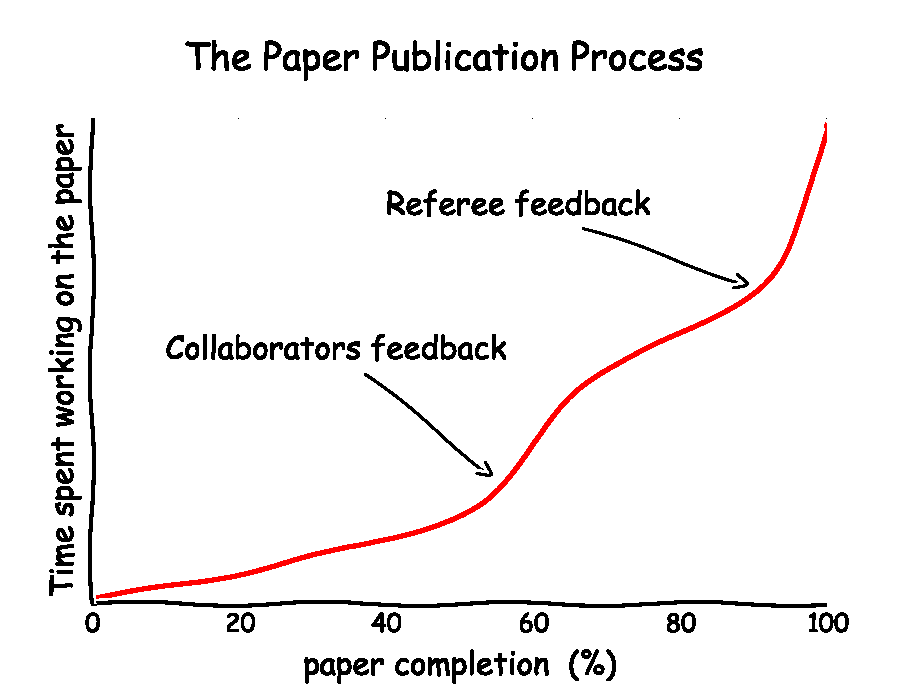
\includegraphics[width=\linewidth, clip]{figs/paperwriting.ps}
\caption{The Paper Publication Process.  The following clause seems to be
  universal: ``The closer you are to finish a paper, the longer it
  takes to make any significant improvement.''  On other news,
  although this figure in particular has a title, in papers, figure titles
  appear as the first sentence fragment of the
  caption, as seen in this caption, rather than at the top of the
  graphic.}
\label{fig:writing}
% SOURCE: /home/patricio/ast/esp01/code/lib/python/xkcd/paperwritting.py
\end{figure}


\subsection{Grammar}
\label{sec:grammar}

And now some grammar: `which' introduces a clause that adds a new fact,
and must be set between commas.  For example: ``There was an earthquake
in Chile, which isn't really any news.''  `That' introduces a clause
that explains or limits, and has no surrounding commas.  For example:
``Class O-stars that lie in the constellation of Orion have small proper
motion.''

Use the ``Oxford'' comma in lists.  For example, ``I love my parents, Lady Gaga, and Humpty Dumpty.'', NOT ``I love my parents, Lady Gaga and Humpty Dumpty.''

Use a hyphen to connect two adjectives acting as a single adjective on
a noun.  You have a bad-pixel map, not a bad pixel map.  The former is
a map of bad pixels.  The latter could be a pixel map, but a bad one.
The hyphen breaks the ambiguity.  However, do {\em not}\/ use a hyphen
between an adverb and an adjective, as the adverb could never modify
the noun and there is no ambiguity: ``We applied a poorly made mask,''
not, ``we applied a poorly-made mask.''  Note that this is a change in
practice from before 2000 or so.  Also, do not hyphenate inside names
or between a number and its units: ``our 3 hour Markov-Chain Monte
Carlo run,'' not ``our 3-hour Markov-Chain Monte-Carlo run.''


\section{SCIENCE}
\label{sec:science}

This section gives a scientific interpretation of the analyzed data.
The \texttt{'\textbackslash micro'} macross provides the unslanted mu,
`{\micro}' to be used for units of values, for example: {\micron} or
{\microbar}.  Another nice feature are \texttt{'\$\textbackslash
  ttt\{n\}\$'} for a 'ten-to-the-n' ($\ttt{n}$) and
\texttt{'\$\textbackslash tttt\{n\}\$'} for 'times-ten-to-the-n'
($\tttt{n}$).

Table \ref{table:parameters} is a table.  Tables are well behaved;
most of the time they appear right (or close to) where you put them.
Figures are not.  The can show up anywhere in the pdf.   Be patient.

\begin{table}[ht]
\centering
\caption{\label{table:parameters} Light curve parameters}
\begin{tabular}{lc}
\hline
\hline
Parameter                           & Value           \\
\hline
Eclipse depth (counts)              & 98.1            \\
Eclipse duration (phase)            & 0.1119          \\
Eclipse mid point (phase)           & 0.5015          \\
Eclipse ingress/egress time (phase) & 0.013           \\
Ramp slope (counts/phase)           & 0.006           \\
System flux (counts)                & 25815           \\
\hline
% SOURCE: /home/patricio/ast/esp01/analyses/ligtcurve/attempt_547/results.txt
\end{tabular}
\end{table}


Deluxe tables, like Table \ref{table:allplanets} are great. If they
are too long, they automatically split and continue in the next
page. Everything looks fine in Aastex6; however, in emulateapj the
format seems to fail.
Deluxe table may be a bit tricky. If you surround it with the table
environment, you can specify where to place them (e.g., top, bottom).
However, if you do, long tables wont automatically break into separate
pages.  So, there is a trade off.

%\begin{table}[t]
% deluxetable works well for aastex6, not so much for emulateapj:
\begin{deluxetable*}{lr@{}lr@{}lrrccrrrccrr}
\tabletypesize{\footnotesize}
%\tablecolumns{14}
%\tablewidth{\textwidth}
\tablecaption{Planets \label{table:allplanets}}

\tablehead{\colhead{Name}                          &
           \multicolumn{2}{c}{Mass}                &
           \multicolumn{2}{c}{Radius}              &
           \colhead{\Teq}                          &
           \colhead{$\Omega$}                      &
           \colhead{$a$}                           &
           \colhead{$M$\sb{s}}                     &
           \colhead{Age}                           &
           \colhead{$\Omega\sb{\rm rot}$}          &
           \colhead{Flux}                          &
           \colhead{$L\sb{\rm h}$}                 &
           \colhead{$L\sb{\rm e}$}                 &
           \colhead{$L\sb{\rm h}$/$L\sb{\rm e}$}   &
           \colhead{Ref.\,\tnm{a}}                 \\
           \colhead{}                              &
           \multicolumn{2}{c}{\mearth}             &
           \multicolumn{2}{c}{\rearth}             &
           \colhead{}                              &
           \colhead{}                              &
           \colhead{}                              &
           \colhead{\msun}                         &
           \colhead{}                              &
           \colhead{$\Omega\sb{\odot}$}            &
           \colhead{erg\,s$\sp{-1}$\,cm$\sp{-2}$}  &
           \colhead{s$\sp{-1}$}                    &
           \colhead{s$\sp{-1}$}                    &
            \colhead{}                              }
\startdata
55 Cnc e      & $ 8.38$ & $\pm 0.39$               & $ 2.08$ & $\pm 0.16$             &         1957 &       15.6 & $0.015$ & $0.91$ & $  10.2$ & $1.4$ & $142697.6$ & $3\times10^{30}$ & $3\times10^{30}$ & $\cdots$ & De11 \\
55 Cnc e      & $ 8.38$ & $\pm 0.39$               & $ 2.08$ & $\pm 0.16$             &         1957 &       15.6 & $0.015$ & $0.91$ & $  10.2$ & $1.4$ & $142697.6$ & $\cdots$ & $\cdots$ & $\cdots$ & De11 \\
55 Cnc e      & $ 8.38$ & $\pm 0.39$               & $ 2.08$ & $\pm 0.16$             &         1957 &       15.6 & $0.015$ & $0.91$ & $  10.2$ & $1.4$ & $142697.6$ & $\cdots$ & $\cdots$ & $\cdots$ & De11 \\
55 Cnc e      & $ 8.38$ & $\pm 0.39$               & $ 2.08$ & $\pm 0.16$             &         1957 &       15.6 & $0.015$ & $0.91$ & $  10.2$ & $1.4$ & $142697.6$ & $\cdots$ & $\cdots$ & $\cdots$ & De11 \\
\enddata
% The minipage environment keeps the table footer within the page
% width when the table occupies the full width.
% Use \vspace to adjust latex quirks with the vertical spacing.
%\begin{minipage}{\textwidth}%\vspace{0.4cm}
\tablenotetext{a}{
Lorem Ipsum is simply dummy text of the printing and typesetting industry. Lorem Ipsum has been the industry's standard dummy text ever since the 1500s, when an unknown printer took a galley of type and scrambled it to make a type specimen book. It has survived not only five centuries, but also the leap into electronic typesetting, remaining essentially unchanged. It was popularised in the 1960s with the release of Letraset sheets containing Lorem Ipsum passages, and more recently with desktop publishing software like Aldus PageMaker including versions of Lorem Ipsum.
}
%\end{minipage}
\end{deluxetable*}
%\end{table}

\subsection{Non-ApJ Templates}
This template is also compatible with other class files (e.g.,
article).  This can come in handy when preparing proposals.
Especially for this case, take a look at the \texttt{top-apj.tex} file
to enable the compact and or bullet-point Refenreces list.

\section{CONCLUSIONS}
\label{sec:conclusions}

These are our conclusions.  Although this example has used a colloquial
dialogue, real papers should use a formal writting style.  After the
conclusions we include some acknowledgments.

Lorem Ipsum is simply dummy text of the printing and typesetting
industry. Lorem Ipsum has been the industry's standard dummy text ever
since the 1500s, when an unknown printer took a galley of type and
scrambled it to make a type specimen book. It has survived not only
five centuries, but also the leap into electronic typesetting,
remaining essentially unchanged. It was popularised in the 1960s with
the release of Letraset sheets containing Lorem Ipsum passages, and
more recently with desktop publishing software like Aldus PageMaker
including versions of Lorem Ipsum.


\acknowledgments

We thank A.\ Friend, B.\ Foe, and an anonymous referee for helpful
discussions and improvements to the paper.  C.\ Scientist provided the
data in table 1.
We thank contributors to SciPy, Matplotlib, and the Python Programming
Language; the free and open-source community; the NASA Astrophysics
Data System; and the JPL Solar System Dynamics group for software and
services.
Part of this work is based on observations made with the
{\em Spitzer Space Telescope}, which is operated by the Jet Propulsion
Laboratory, California Institute of Technology under a contract with
NASA.
Support for this work was provided by NASA through an award
issued by JPL/Caltech and through the NASA Science Mission
Directorate's Astrophysics Data Analysis Program, grant
XXY00ZZZ1110.
Jill held a NASA Earth and Space Science Fellowship.  Tom was a
Fulbright Scholar.  Get the right wording from each entity you must
acknowledge.  This is very important!!!

\bibliography{template}

\begin{appendices}

\section{BAYESIAN CREDIBLE REGION}
\label{sec:CredRegion}

In the Bayesian context, given the posterior probability density,
$p(\theta|{\bf D})$, of a parameter, $\theta$, given the dataset,
${\bf D}$, the highest posterior density region (or credible
region), $R$, is defined by
\begin{equation}
C = \int\sb{R} {\rm d}\theta\;p(\theta|{\bf D})
\label{eq:CredRegion}
\end{equation}
where C is the probability contained in the credible region.  The
region $R$ is selected such that the posterior probability of any
point inside $R$ is larger than that of any point outside.  We like
Eq.\ (\ref{eq:CredRegion}).

\end{appendices}

\end{document}
